\documentclass{article}


\usepackage{fancyhdr}
\usepackage{extramarks}
\usepackage{amsmath}
\usepackage{amsthm}
\usepackage{amsfonts}
\usepackage{tikz}
\usepackage[plain]{algorithm}
\usepackage{algpseudocode}
\usepackage{enumerate}
\usepackage{tikz}
\usepackage{listings}
\usepackage{hyperref}
\usepackage{subfigure}
\usepackage[graphicx]{realboxes}
\usepackage{xcolor}
\usepackage{color}



% 代码块高级设置
\lstset{
basicstyle=\footnotesize,                 % 设置整体的字体大小
showstringspaces=false,                     % 不显示字符串中的空格
frame=single,                               % 设置代码块边框
numbers=left,                               % 在左侧显示行号
% numberstyle=\footnotesize\color{gray},    % 设置行号格式
numberstyle=\color{darkgray},               % 设置行号格式
backgroundcolor=\color{white},              % 设置背景颜色
keywordstyle=\color{blue},                  % 设置关键字颜色
commentstyle=\it\color[RGB]{0,100,0},       % 设置代码注释的格式
stringstyle=\sl\color{red},                 % 设置字符串格式
}

\hypersetup{hidelinks,
	colorlinks=true,
	allcolors=black,
	pdfstartview=Fit,
	breaklinks=true}

%
% Basic Document Settings
%  

\topmargin=-0.45in
\evensidemargin=0in
\oddsidemargin=0in
\textwidth=6.5in
\textheight=9.0in
\headsep=0.25in

\linespread{1.1}

\pagestyle{fancy}
\lhead{}
\chead{\hmwkClass : \hmwkTitle}
\rhead{\firstxmark}
\lfoot{\lastxmark}
\cfoot{\thepage}

\renewcommand\headrulewidth{0.4pt}
\renewcommand\footrulewidth{0.4pt}

\setlength\parindent{0pt}



%
% Homework Details
%   - Title
%   - Due date
%   - Class
%   - Instructor
%   - Class number
%   - Name
%   - Student ID

\newcommand{\hmwkTitle}{Problem Set 2 Document}
\newcommand{\hmwkDueDate}{Nov 1st}
\newcommand{\hmwkClass}{Parallel Computing}
\newcommand{\hmwkClassInstructor}{Professor Rui Fan}

% 正式选课名单确定之后,根据通知填写所在班级编号

\newcommand{\hmwkAuthorName}{Zhenghong Yu}
\newcommand{\hmwkAuthorMail}{yuzhh1@shanghaitech.edu.cn}
\newcommand{\hmwkAuthorID}{2020533156}


%
% Title Page
%

\title{
    \vspace{2in}
    \textmd{\textbf{\hmwkClass:\\  \hmwkTitle}}\\
    \normalsize\vspace{0.1in}\small{Due\ on\ \hmwkDueDate\ at 23:59 }\\
   \vspace{2in}
}

\author{
    Mailbox: \hmwkAuthorMail\\
	Student ID: \hmwkAuthorID\\
    Student Name: \hmwkAuthorName}
\date{}




\begin{document}

\maketitle
\pagebreak
\tableofcontents

\pagebreak





\section{Problem 1}
Given a balanced binary tree, describe a procedure to perform all-to-all 
broadcast that takes time $(t_{s} + t_{w}mp/2)\log p$ for $m$-word messages on $p$ nodes. Assume that only the leaves of the tree contain nodes, and that an exchange of 
two $m$-word messages between any two nodes connected by bidirectional 
channels takes time $t_{s} + t_{w}mk$ if the communication channel (or a part of it) is 
shared by $k$ simultaneous messages.\\\\
\textbf{Solution: }\\\\
\begin{center}
    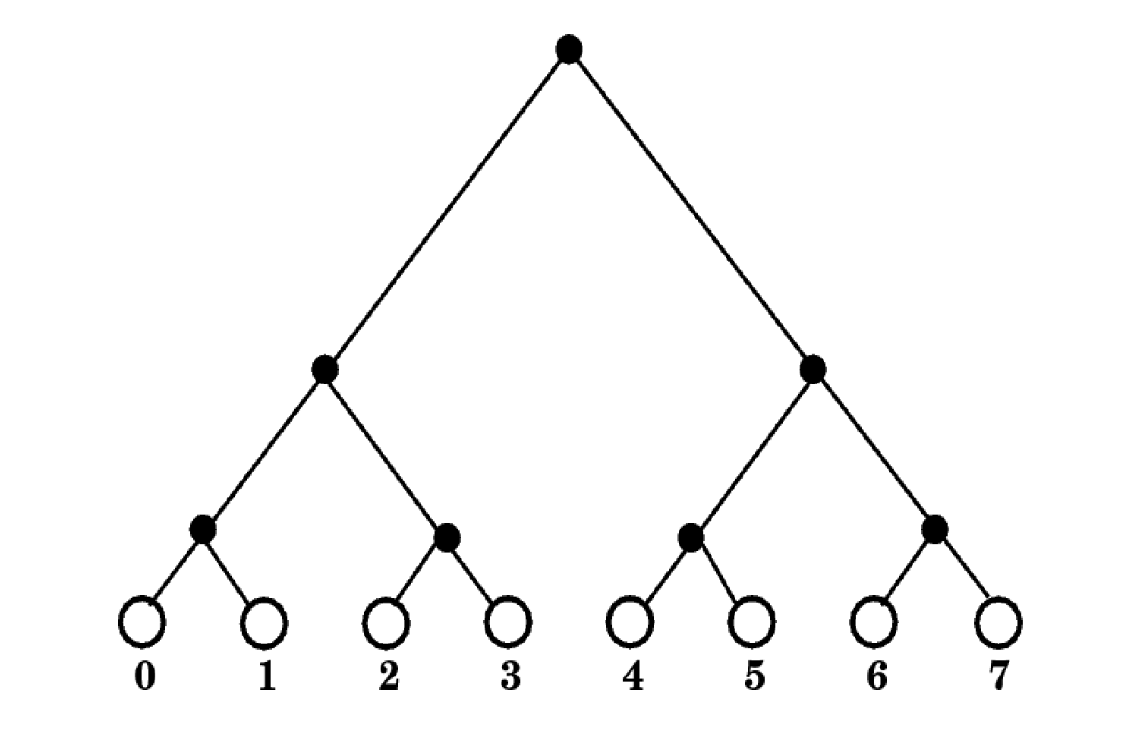
\includegraphics[scale = 0.25]{p1.png}\\
\end{center}
Given picture above, initially, every nodes hold a $m$-word message.\\
First, copy the message of every two nodes in different subtrees and transfer it to each other in the bi-directional channel. All communication take use of path through root, thus the workload is $mp/2$, thus the cost is $t_{1}=t_{s}+t_{w}mp/2$.\\
Then, run the similar procedures in the two subtrees recursively. The workload of every channels is $2^imp/(2*2^i)=mp/2$, thus the cost is still $t_{i}=t_{s}+t_{w}mp/2$. 
Finally, we will run $\log p$ recursion. The finally cost is, $(t_{s} + t_{w}mp/2)\log p$.
\pagebreak
\section{Problem 2}
Consider the following sequential rank sort algorithm for n values assuming no 
duplicate values: 
\begin{lstlisting}[language=c++]
for (i = 0; i < n; i++) { 
    x = 0; 
    for (j = 0; j < n; j++) 
        if (a[i] > a[j]) x++; 
    b[x] = a[i]; 
} 
\end{lstlisting}
\subsection{Question 1}
Rewrite this as a parallel algorithm using OpenMP assuming that $p < n$ threads are used. Clearly indicate the use of private and shared variables and the schedule type.
\\\textbf{Solution: }
\begin{lstlisting}[language=c++]
#pragma omp parallel for schedule(static) private(x,j) shared(i,a,b)
{
    for(i = 0; i < n; i++)
    {
        x = 0;
        for(j = 0; j < n; j++)
            if(a[i] > a[j]) x++;
        b[x] = a[i];
    }
}
\end{lstlisting} 
\subsection{Question 2}
Modify the OpenMP code in part (a) to handle duplicates in the list of 
values, i.e. to sort into non-decreasing order. For example, the list of values 
[3, 5, 7, 5, 7, 9, 2, 3, 6, 7, 8, 1] should give the sorted list [1, 2, 3, 3, 5, 5, 6, 
7, 7, 7, 8, 9]. 
\\\textbf{Solution: }
\begin{lstlisting}[language=c++]
#pragma omp parallel for schedule(static) shared(a,b,i) private(x,j,d)
{
    for(i = 0; i < n; i++)
    {
        x = 0;
        d = 0;
        for(j = 0; j < n; j++)
            if(a[i] > a[j]) rank++;
            else if((a[i] == a[j]) && (i > j)) d++;
        b[x + d] = a[i];
    }
}
\end{lstlisting} 

\pagebreak

\section{Problem 3}
The following sequential code calculates a triangular matrix using a function \textbf{calc(i,j)}, which has no data dependences and requires a constant (but large) amount of computation. 
\begin{lstlisting}[language=c++]
for (i = 0; i < n; i++) 
    for (j = 0; j <= i; j++) 
        a[i,j] = calc(i,j);
\end{lstlisting}
By inserting OpenMP directives into the sequential code, show how the 
following schemes for assigning work to threads may be implemented on a 
shared memory parallel architecture, commenting on the efficiency of each 
scheme: 
\subsection{Question 1}
A static block assignment of contiguous rows to threads. 
\\\textbf{Solution: }
\begin{lstlisting}[language=c++]
#pragma omp parallel for schedule(static) shared(a) private(j)
{
    for(i = 0; i < n; i++)
    {
        for (j = 0; j <= i; j++) 
            a[i,j] = calc(i,j);
    }
}
\end{lstlisting}
The load balance of threads is poor, since quite different amount of works are allocated to different threads.
\subsection{Question 2}
A static cyclic assignment of single rows to threads. 
\\\textbf{Solution: }
\begin{lstlisting}[language=c++]
#pragma omp parallel for schedule(static,1) shared(a,i) private(j)
{
    for(i = 0; i < n; i++)
    {
        for (j = 0; j <= i; j++) 
            a[i,j] = calc(i,j);
    }
}
\end{lstlisting}
Better than the previous one, different parts of matrix are sampled to a thread. It's more load balanced. The performance is depend on the chunk size.
\subsection{Solution: }
A dynamic assignment of single rows to threads. 
\\\textbf{Solution: }
\begin{lstlisting}[language=c++]
#pragma omp parallel for schedule(dynamic,1) shared(a,i) private(j)
{
    for(i = 0; i < n; i++)
    {
        for (j = 0; j <= i; j++) 
            a[i,j] = calc(i,j);
    }
}
\end{lstlisting}
It should be close to the previous situation, but it might be slower due to the overhead of dynamic scheduling, since the triangular is high structured.

\section{Problem 4}
The $Back Substitution$ algorithm solves a set of linear equations in upper (or 
lower) triangular form, as shown in Figure Q4a. A sequential algorithm to solve 
such a set of linear equations is given in Figure Q4b. Design a parallel algorithm 
for a shared memory architecture and express it using OpenMP assuming that p 
< n threads are used. What schedule type would you use?
\begin{center}
    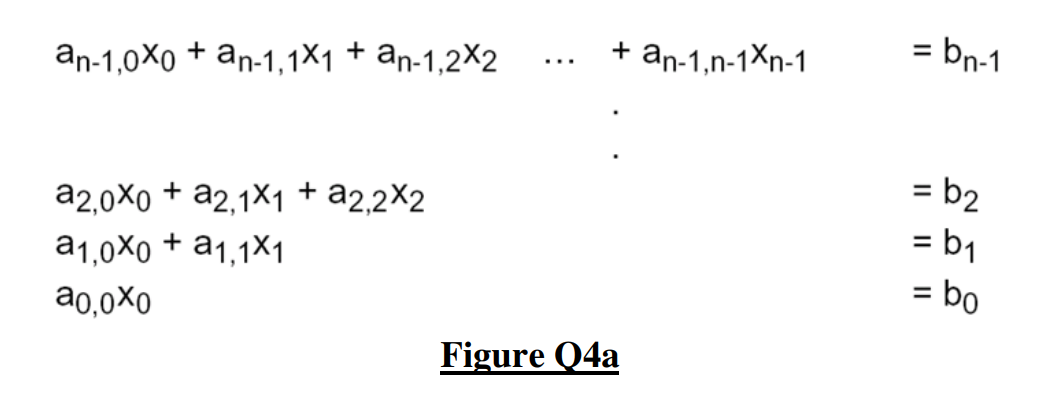
\includegraphics[scale = 0.25]{q4.png}\\
\end{center}
\begin{lstlisting}[language=c++]
/* Back Substitution */
for (i = 0; i < n; i++) { 
    x[i] = b[i]/a[i][i]; 
    for (j = i+1; j < n; j++) { 
        b[j] = b[j] - a[j][i]*x[i]; 
        a[j,i] = 0; 
    } 
}
\end{lstlisting}
\textbf{Solution: }
\begin{lstlisting}[language=c++]
/* Back Substitution */
for (i = 0; i < n; i++) { 
    x[i] = b[i]/a[i][i];
    #pragma omp parallel for schedule(static) 
    for (j = i+1; j < n; j++) { 
        b[j] = b[j] - a[j][i]*x[i]; 
        a[j,i] = 0; 
    } 
}
\end{lstlisting}
Since the back substitution is sequential, solve $x_{i}$ depends on solving $x_{i-1}$, our strategy is to assign the iterations of inner loop to different threads to accelerate. A static scheduling is suitable, since the workloads of iterations are approxiately the same.\\
Rows i>j will have approxiately the same work so can use static block schedule.

\pagebreak

\section{Problem 5}
GPU computing has been used to speed up many real-world applications. 
However, not all applications are suitable for GPU acceleration. Consider the 
following operations / applications and decide whether each is suitable for GPU 
acceleration or not. Briefly justify your answer. Assume all the input data are 
initially in the main memory.
\subsection{Question 1}
Matrix multiplications on two matrices A and B, each of size 32000 by 32000.
\\\textbf{Solution: }\\
Suitable, it has large amounts of parallelism. Threads perform the same operations and are load balanced. Memory accesses can be made efficient with tiling.
\subsection{Question 2}
Matrix multiplications on two matrices A and B, each of size 32 by 32.
\\\textbf{Solution: }\\
Not that suitable, problem is too small, not enough work to pay for the overhead of kernel launch and not enough parallelism to occupy device.
\subsection{Question 3}
Binary search on a sorted array with 1 billion elements.
\\\textbf{Solution: }\\
Unsuitable,there's no parallelism, can't occupy GPU. Thread divergance. Nocoalesced memory accessed.
\subsection{Question 4}
Binary search on a sorted array with 1 thousand elements. 
\\\textbf{Solution: }\\
Not that unsuitable, also no parallelism, and threads diverge. But this time, we can do many binary searches in parallrl, can keep array in shared memory to avoid uncoalesced memory access.

\pagebreak

\section{Problem 6}
\subsection{Question 1}
Consider the following CUDA kernel for copying a matrix \textbf{idata} to another matrix \textbf{odata}. One reason for doing this is simply to test the memory bandwidth achievable on a GPU. At a high level, the kernel launches a 2D grid of thread 
blocks each of size \textbf{[TILE\_DIM, BLOCK\_ROWS]}, and each thread block copies 
a tile of values of size \textbf{TILE\_DIM x TILE\_DIM} from idata to odata. 
Suggested values are \textbf{TILE\_DIM=32}, \textbf{BLOCK\_ROWS=8}.\\
Give a detailed explanation of how the code works. Given an \textbf{NX x NY} matrix, 
how many thread blocks should be launched? Why do we want to set 
\textbf{BLOCK\_ROWS} less than \textbf{TILE\_DIM}? What does width represent? Why does the loop iterate over the variable $j$? What do the index calculations like $x*width+(y+j)$ do? 
\begin{lstlisting}[language=c++]
__global__ void copy(float *odata, const float *idata)
{
    int x = blockIdx.x * TILE_DIM + threadIdx.x;
    int y = blockIdx.y * TILE_DIM + threadIdx.y;
    int width = gridDim.x * TILE_DIM;
    for (int j = 0; j < TILE_DIM; j+= BLOCK_ROWS)
        odata[(y+j)*width + x] = idata[(y+j)*width + x];
}
\end{lstlisting}
\textbf{Solution: }\\
There are $(NX/TITL\_DIM)*(NY/TITLE\_DIM)$ blocks should be launched. There are $(TILE\_DIM/BLOCK\_ROWS)*TILE\_DIM = 128$ threads should be launched per block.\\
If \textbf{BLOCK\_ROWS} is larger than \textbf{TILE\_ROWS}, every thread will copy only one element of data, which will cause too much overhead and thus low efficiency.\\
Width means padded width of the source and target data.\\
$j$ means the iterate step over the row dimension. This is because it cause contiguous threads to load and store contiguous data, the reads from idata and writes to odata thus are coalsced.\\
$x*width+(y+j)$ means the transposed id of $(y+j,x)$
\subsection{Question 2}
We now modify the above kernel to transpose matrix idata to another matrix odata. Again, explain in detail how the code works. Do you expect the kernel to achieve good performance (compared to copying the matrix) when transposing a large matrix? Explain your reasoning. 
\begin{lstlisting}[language=c++]
__global__ void transposeNaive(float *odata, const float *idata)
{
    int x = blockIdx.x * TILE_DIM + threadIdx.x;
    int y = blockIdx.y * TILE_DIM + threadIdx.y;
    int width = gridDim.x * TILE_DIM;
    for (int j = 0; j < TILE_DIM; j+= BLOCK_ROWS)
        odata[x*width + (y+j)] = idata[(y+j)*width + x];
\end{lstlisting}
\textbf{Soluton: }\\
The question answer is similar to the previous question above, except swapping the index of odata. I expect the kernel not achieve good performance, since the write operation are not coalsced, the transpose performance will be much lower than copy transpose.












\end{document}
